% Anonymous BlackboxNLP 2026 revision of the ARR-reviewed manuscript

\documentclass[11pt]{article}
\usepackage[review]{acl}
\usepackage{times}
\usepackage{latexsym}
\usepackage[T1]{fontenc}
\usepackage[utf8]{inputenc}
\usepackage{microtype}
\usepackage{inconsolata}
\usepackage{graphicx}
\usepackage{amsmath}
\usepackage{amssymb}
\usepackage{booktabs}
\usepackage{multirow}
\usepackage{xcolor}
\usepackage{url}

\newcommand{\fep}{\textsc{FEP}}

\title{First Is Not Stable: Auditing Layerwise Vocabulary Readout in Language Models}
\author{Anonymous ACL submission}

\begin{document}
\maketitle

\begin{abstract}
Vocabulary projections are often used to ask when a chosen answer token becomes visible inside a language model. A common scalar summary---the first layer at which the token enters the vocabulary top-$k$---has two failure modes: a token that never enters top-$k$ can be conflated with final-layer entry, and a transient entry can be mistaken for stable readout. We audit this measurement and introduce a trajectory-aware protocol that separates first entry, persistent entry, any later absence, final disappearance, and right-censored non-entry. Across 817 TruthfulQA questions and six 6.9--14B base models, 21.9--31.1\% of first answer tokens never enter the top-10, while 15.2--48.0\% enter and are absent again at least once later. The largest rate is fragile: Gemma's 48.0\% is dominated by one penultimate-layer readout and falls to 23.4\% when that observation is treated as missing. Controls on MMLU and SST-2 further show strong task-format dependence. On SST-2, Mistral and Pythia reach 86.9\% and 80.8\% candidate-choice accuracy while the correct label appears in the final full-vocabulary top-10 for 0\% of examples. We therefore argue that layerwise vocabulary rank is a property of a model--prompt--target interface, not a direct measure of knowledge storage, causal use, or even candidate-task competence. The supplementary artifact contains corrected code, per-layer ranks, audit checks, and tests.
\end{abstract}

\section{Introduction}
Projecting an intermediate residual state through a language model's output head gives an intuitive view of how token predictions evolve with depth. This ``logit lens'' has supported analyses of prediction construction \citep{nostalgebraist2020logitlens,geva2022transformer}, factual decoding \citep{chuang2024dola}, and early exit \citep{elhoushi2024layerskip}. Its appeal is precisely its simplicity: for a target token, one may record the earliest layer at which it enters the top-$k$ vocabulary predictions.

That scalar is easy to misinterpret. First, targets that never enter top-$k$ are right-censored observations; assigning them the final layer invents an event that did not occur. Second, vocabulary-rank trajectories need not be monotone. A target may enter, leave, and re-enter the top-$k$, so first entry need not mark a stable transition. Third, the rank is taken over the full vocabulary even when a task evaluates a small candidate set. It can therefore reflect answer formatting and prompt calibration rather than task competence.

We present a measurement audit and a corrected trajectory protocol. We use \emph{factual emergence point} (FEP) as shorthand for the first-entry statistic: when does a specified target first become directly readable through the model's native output head? We explicitly distinguish first entry, persistent entry, any later absence, final disappearance, and never observed. We also extract the target by jointly tokenizing prompt and continuation, avoiding tokenizer-boundary changes.

Our experiments reveal a more heterogeneous picture than a single ``late emergence'' statistic suggests. On TruthfulQA, final top-10 visibility spans 64.7--71.7\%, yet the paths differ sharply. Pythia-6.9B first exposes observed targets at 45.4\% depth on average but has a 28.4\% any-later-absence rate. Gemma-7B first exposes them at 84.9\% depth and has a raw rate of 48.0\%, but this headline is dominated by an isolated penultimate-layer readout collapse. Qwen2.5-7B and 14B show similar normalized profiles, but this within-family comparison does not identify a scaling law.

Task-format controls are equally consequential. Qwen2.5-7B exposes every correct MMLU option label in its final top-10, compared with 64.7\% of TruthfulQA answer tokens. Across five models on SST-2, candidate accuracy and free-vocabulary visibility can diverge almost completely. These results narrow the interpretation of vocabulary projections and provide concrete reporting requirements for future layerwise analyses.

Our contributions are:
\begin{itemize}
    \item a censoring- and trajectory-aware definition of layerwise target readout, with explicit token-boundary and final-logit consistency checks;
    \item a complete rerun on six models and three task settings, releasing per-sample ranks rather than only aggregate means;
    \item evidence that first visibility, persistence, and task competence are distinct, together with a minimal reporting checklist intended to prevent over-interpretation.
\end{itemize}

\section{Related Work}
\paragraph{Vocabulary-space projections.}
The logit lens applies the output unembedding to intermediate states \citep{nostalgebraist2020logitlens}. \citet{geva2022transformer} study how feed-forward updates promote vocabulary concepts. Learned transformations reduce the distribution mismatch between intermediate and final representations \citep{belrose2023tuned,yomdin2024jump}, while Future Lens decodes later tokens from a single hidden state \citep{pal2023future}. These methods underline that a raw native-unembedding projection is one readout choice, not a representation-completeness test. Layerwise decoding may also be non-monotone, multilingual trajectories may pass through an English-biased concept region, and spectral components can be poorly represented by a simple token ranking \citep{wendler2024llamas,cancedda2024spectral,nguyen2026iglens}. Recent work models logits across depth: \citet{he2025delta} extrapolate late-layer trajectories for decoding, while \citet{jung2026tracing} aggregate adjacent-layer logit-update vectors into dataset-level geometric summaries. We do not claim that non-monotonicity is new. Our narrower contribution is an event-level audit of a fixed raw projection: explicit censoring and persistence semantics, token-boundary and native-logit checks, single-readout sensitivity, and separation of full-vocabulary visibility from candidate competence.

\paragraph{Factual recall and causal localization.}
Factual recall involves distributed stages and causally important intermediate modules \citep{meng2022locating,geva2023dissecting}. Model editing work identifies parameters that can alter associations \citep{meng2022mass}. A token becoming top-$k$ under an output projection neither establishes where its association is stored nor when it first affects computation. We use ``readout'' or ``visibility'' throughout for this reason.

\paragraph{Decoding and early exit.}
DoLa contrasts layer distributions to improve factual decoding \citep{chuang2024dola}; early-exit methods train or detect usable intermediate predictions \citep{elhoushi2024layerskip}. These methods care about intermediate predictions but have different operational objectives. Our metrics diagnose a fixed model under a fixed prompt and target; they do not themselves provide an exit rule or intervention.

\section{Measurement Protocol}
\subsection{Prompt-conditioned target alignment}
For prompt string $p_i$ and gold continuation $a_i$, we insert exactly one leading space before the stripped continuation and tokenize $p_i+a_i$ jointly. We require that tokenizing $p_i$ alone produces an exact prefix of this sequence. The first continuation token is the target $y_i$. This matters because tokenizing $a_i$ in isolation can produce a different first token at the boundary.

Let $h_{i,l}$ be the residual state at the final prompt position after transformer block $l$, for $l\in\{1,\ldots,L\}$. We apply the model's native final normalization and unembedding:
\begin{equation}
z_{i,l} = W_U\,\mathrm{Norm}_{\mathrm{final}}(h_{i,l}) + b_U,
\end{equation}
and let $r_{i,l}$ be the zero-based vocabulary rank of $y_i$. At $l=L$, we verify that the reprojected logits preserve native final top-$k$ membership and differ by at most 0.25 in maximum absolute logit value. Failed samples are retained in an explicit failure log, not silently dropped; all canonical runs reported here have zero failures.

\subsection{Trajectory-aware events}
For threshold $k$, define $b_{i,l}=\mathbb{1}[r_{i,l}<k]$. We report:
\begin{align}
F_i(k) &= \min\{l:b_{i,l}=1\}, \\
P_i(k) &= \min\{l:\forall m\ge l,\ b_{i,m}=1\}.
\end{align}
$F_i$ is undefined when the target never enters top-$k$; $P_i$ is defined only when it is present at the final layer. We additionally report $N_i=\mathbb{1}[\sum_l b_{i,l}=0]$, any-gap dropout $D_i=\mathbb{1}[\exists l<m: b_{i,l}=1\land b_{i,m}=0]$, and final disappearance $E_i=\mathbb{1}[F_i\text{ defined}\land b_{i,L}=0]$. Thus $D_i$ counts any later absence even if the target re-enters, whereas $E_i$ is the stricter entered-then-absent-at-output event. Means of $F_i/L$ are conditional on observed entries; means of $P_i/L$ are conditional on final presence. We always report their denominators alongside unconditional non-entry and final-presence rates.

This decomposition prevents three different samples---never observed, final-layer first entry, and early-but-transient entry---from receiving the same scalar value.

\section{Experimental Setup}
\paragraph{Models.}
We evaluate Qwen2.5-7B and 14B \citep{qwen2024qwen25}, Llama-3.1-8B \citep{dubey2024llama3}, Mistral-7B-v0.1 \citep{jiang2023mistral}, Pythia-6.9B \citep{biderman2023pythia}, and Gemma-7B \citep{gemma2024}. All are base models. Model family, tokenizer, training data, architecture, and parameter count are confounded; comparisons are descriptive.

\paragraph{Tasks and targets.}
TruthfulQA uses all 817 questions and the first token of the reference best-answer continuation \citep{lin2022truthfulqa}. This is deliberately an answer-prefix audit: 97.9--99.1\% of references are multi-token under the six tokenizers, and 63.8\% of targets belong to the ten most frequent lexical first-token types (e.g., \emph{No}, \emph{The}, and \emph{I}). It does not measure whole-answer semantics. For MMLU, we sample 1,200 examples balanced across 24 subjects and target the correct option label among A/B/C/D \citep{hendrycks2021mmlu}. For SST-2, we use all 872 validation examples and target the label token \texttt{negative} or \texttt{positive} \citep{socher2013sst}. Candidate accuracy is computed by comparing only the task's permitted label continuations; it is deliberately separated from rank over the full vocabulary.

\paragraph{Implementation.}
Unless specified otherwise, $k=10$. Inference uses bfloat16 on one NVIDIA H20 with Python 3.12.13, PyTorch 2.10.0, Transformers 4.48.3, and CUDA 12.8. Artifacts contain prompts, aligned token IDs, ranks and probabilities at every layer, native-logit audit fields, failure records, and SHA-256 checksums. Pure alignment, censoring, persistence, and aggregation functions have CPU unit tests.

\section{TruthfulQA Results}
\begin{table*}[t]
\centering\small
\resizebox{\textwidth}{!}{%
\begin{tabular}{lrrrrrrr}
\toprule
Model & $L$ & Ever $\uparrow$ & Never $\downarrow$ & Final $\uparrow$ & Any gap $D$ $\downarrow$ & Final loss $E$ $\downarrow$ & First / Persistent depth \\
\midrule
Qwen2.5-7B  & 28 & 68.9 & 31.1 & 64.7 & 18.8 & 4.2 & .824 / .876 \\
Qwen2.5-14B & 48 & 71.2 & 28.8 & 67.7 & 16.8 & 3.5 & .872 / .900 \\
Llama-3.1-8B & 32 & 73.8 & 26.2 & 71.7 & 15.2 & 2.1 & .833 / .865 \\
Mistral-7B & 32 & 73.2 & 26.8 & 67.9 & 18.5 & 5.3 & .788 / .835 \\
Pythia-6.9B & 32 & 78.1 & 21.9 & 71.1 & 28.4 & 7.0 & .454 / .615 \\
Gemma-7B & 28 & 76.5 & 23.5 & 71.7 & 48.0 & 4.8 & .849 / 1.000 \\
\bottomrule
\end{tabular}
}
\caption{Corrected top-10 trajectories on 817 TruthfulQA examples. Percentages use all examples. Any gap counts a later absence even after re-entry; final loss requires absence at the output. First depth is conditional on ever-observed targets; persistent depth is conditional on final presence. Wilson 95\% intervals for all rates have half-width at most 3.3 points; full intervals are released.}
\label{tab:truthful}
\end{table*}

\begin{figure*}[t]
\centering

\includegraphics[width=\textwidth]{figures/corrected_truthfulqa_trajectories.pdf}
\caption{TruthfulQA top-10 trajectories. Left: fraction of target tokens in the vocabulary top-10 at each normalized depth. Right: right-censoring and non-monotonicity are both substantial. Pythia's early visibility and Gemma's penultimate-layer dip show why first entry alone is insufficient.}
\label{fig:truthful-trajectories}
\end{figure*}

Table~\ref{tab:truthful} replaces a single ``late'' rate with distinct events. Final visibility spans seven points across models, but first-entry depth varies from .454 to .872. Pairwise exact McNemar tests on final visibility remain significant for 3/15 pairs under Holm family-wise control and 9/15 under Benjamini--Hochberg FDR control. The path differences are stronger: exact sign tests on first-entry depth, restricted to items observed by both models, survive Holm correction for 10/15 pairs. For Gemma versus Pythia, the jointly observed means are .840 versus .446 ($n{=}567$, adjusted $p<10^{-100}$). These post-hoc tests support different paths without establishing an architecture effect. Full pairwise results are released.

\paragraph{Early does not mean stable.}
Pythia has the earliest conditional first entry (14.53/32 layers), yet 28.4\% of all targets are absent at least once later and persistent entry moves to 19.67/32. Gemma's raw trajectory is more extreme: observed targets first enter at 23.77/28 and 48.0\% have a later absence. These are any-gap rates, not final failures: only 7.0\% and 4.8\%, respectively, enter and end absent. A scalar first entry calls all of these targets ``observed'' while missing their different dynamics.

\subsection{Sensitivity to a single readout}
\begin{table}[t]
\centering\small
\resizebox{\columnwidth}{!}{%
\begin{tabular}{lrrrr}
\toprule
Model & Flagged & Prev. & Raw $D$ & Missing $D$ \\
\midrule
Llama-3.1-8B & 25/32 & 30.0 & 15.2 & 12.1 \\
Mistral-7B & 10/32 & 1.8 & 18.5 & 17.0 \\
Qwen2.5-14B & 47/48 & 63.6 & 16.8 & 14.6 \\
Qwen2.5-7B & 27/28 & 53.5 & 18.8 & 16.6 \\
Gemma-7B & 27/28 & 0.5 & 48.0 & 23.4 \\
Pythia-6.9B & 9/32 & 29.3 & 28.4 & 25.9 \\
\bottomrule
\end{tabular}
}
\caption{Leave-one-readout-out sensitivity (percent). Prev. is top-10 prevalence at the flagged layer; Missing $D$ treats it as unobserved. The layer is selected post hoc, so this is a fragility diagnostic, not a corrected lens.}
\label{tab:layer-sensitivity}
\end{table}

Gemma's 48.0\% rate is concentrated at layer 27/28: top-10 prevalence falls from 37.7\% to 0.5\% and rebounds to 71.7\%, while the median target rank changes $36\!\rightarrow\!1373\!\rightarrow\!3$. All 392 Gemma samples counted as dropout are absent at this readout. Treating it as missing reduces dropout to 23.4\% and moves mean persistent depth from 1.000 to .906 on the original 28-layer coordinate. Its 24.6-point reduction is 10.1 times Gemma's second-largest layer effect; the largest reduction for any other model is 3.1 points (Table~\ref{tab:layer-sensitivity}). Three of six post-hoc flagged layers are penultimate, motivating explicit sensitivity reporting near the native output. This is evidence that raw-projection trajectory summaries can be dominated by one observation, not evidence that the intervening transformer block destroys and reconstructs the underlying information.

\paragraph{Never observed is not final-layer entry.}
Between 21.9\% and 31.1\% of targets are never top-10 under the native vocabulary projection. Treating these as layer $L$ would inflate conditional depths and create a spurious mass of final-layer events. Conversely, targets genuinely entering at $L$ remain observed events. Our artifacts keep the two states separate as \texttt{null} and $L$.

\paragraph{Within-family scale comparison.}
Qwen2.5-7B and 14B have close point estimates for ever-observed rates (68.9\% vs. 71.2\%) and persistent depths (.876 vs. .900). With only two sizes and no equivalence margin, we make no profile-equivalence or scaling claim.

\subsection{Sensitivity to the vocabulary threshold}
\begin{table}[t]
\centering\small
\begin{tabular}{rrrrr}
\toprule
$k$ & Ever & Never & Final & First / Persist. \\
\midrule
1   & 27.3 & 72.7 & 19.7 & .880 / .941 \\
3   & 49.2 & 50.8 & 40.0 & .850 / .905 \\
5   & 57.5 & 42.5 & 50.9 & .836 / .890 \\
10  & 68.9 & 31.1 & 64.7 & .824 / .876 \\
20  & 76.9 & 23.1 & 74.7 & .800 / .859 \\
50  & 85.9 & 14.1 & 84.7 & .758 / .831 \\
100 & 91.8 & 8.2  & 90.2 & .710 / .806 \\
\bottomrule
\end{tabular}
\caption{Threshold sensitivity for Qwen2.5-7B on TruthfulQA (percent except normalized depths). Conclusions depend quantitatively on $k$, so a single threshold should not be presented as intrinsic.}
\label{tab:topk}
\end{table}

Increasing $k$ smoothly reduces censoring and shifts entry earlier (Table~\ref{tab:topk}); there is no threshold-independent ``emergence layer.'' Even at $k=100$, however, observed targets first enter at 71.0\% depth and stabilize at 80.6\% depth on average. The appropriate conclusion is therefore conditional: direct vocabulary readout tends to improve late for this prompt and target, while its apparent timing is threshold-dependent.

\section{The Interface Is Part of the Measurement}
\subsection{Controlled prompt-template variation}
\begin{table}[t]
\centering\small
\resizebox{\columnwidth}{!}{%
\begin{tabular}{lrrrr}
\toprule
Template & Ever & Final & Any gap & First / Persist. \\
\midrule
\texttt{Q/A} & 68.9 & 64.7 & 18.8 & .824 / .876 \\
\texttt{Question/Answer} & 69.6 & 65.7 & 22.3 & .818 / .865 \\
Truthful instruction & 77.2 & 74.4 & 16.6 & .811 / .842 \\
\bottomrule
\end{tabular}
}
\caption{Qwen2.5-7B on the same 817 TruthfulQA questions and targets under three prompt templates (percent except normalized depths).}
\label{tab:prompts}
\end{table}

The abbreviated and expanded neutral templates give similar results (paired exact McNemar $p=.54$ for final visibility), but adding ``Answer the following question truthfully'' increases final top-10 visibility by 9.7 points ($110$ gains vs. $31$ losses, $p<10^{-10}$) and shifts persistent entry earlier (Table~\ref{tab:prompts}). The model, questions, targets, and threshold are held fixed. Vocabulary readout is therefore not a model-only profile; semantically relevant prompt wording can materially reshape it.

\begin{figure}[t]
\centering
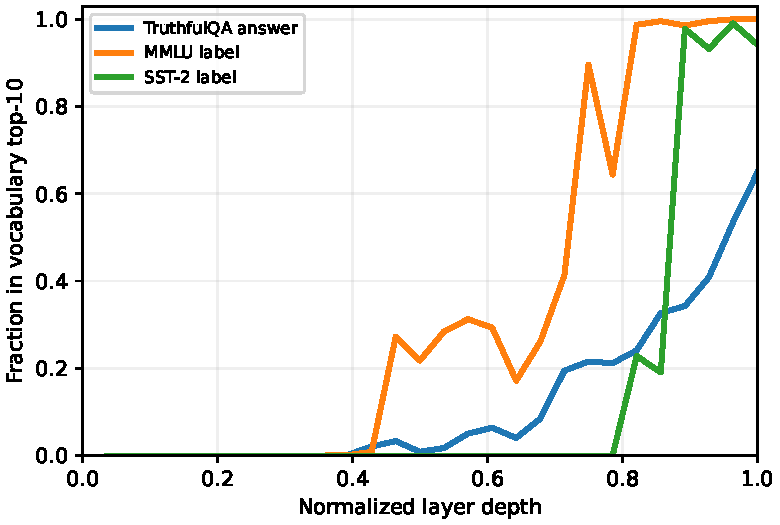
\includegraphics[width=\columnwidth]{figures/corrected_task_format.pdf}
\caption{Qwen2.5-7B top-10 prevalence for three targets. MMLU option labels become visible much earlier than TruthfulQA answer tokens; SST-2 labels change sharply near the output.}
\label{fig:task-format}
\end{figure}

\subsection{MMLU option labels}
Qwen2.5-7B reaches 72.0\% candidate accuracy on 1,200 MMLU examples. Every correct A/B/C/D label both enters and ends in the full-vocabulary top-10. Nevertheless, 52.9\% have at least one later absence before returning; group rates range from 47.6\% to 63.6\%. Conditional first and persistent depths are .646 and .731, respectively. Across STEM, humanities, social sciences, and other subjects, final visibility remains 100\% while candidate accuracy ranges from 63.1\% to 80.0\%. Thus, visibility of the correct label is not correctness, and final presence alone also hides trajectory instability.

\subsection{SST-2: candidate competence without free readout}
\begin{table}[t]
\centering\small
\begin{tabular}{lrrrr}
\toprule
Model & Acc. & Ever & Final & Any gap \\
\midrule
Qwen2.5-7B & 91.6 & 99.5 & 94.3 & 20.5 \\
Mistral-7B & 86.9 & 48.9 & 0.0 & 48.9 \\
Llama-3.1-8B & 73.2 & 44.5 & 35.1 & 28.4 \\
Pythia-6.9B & 80.8 & 0.0 & 0.0 & 0.0 \\
Gemma-7B & 69.8 & 2.1 & 2.1 & 0.0 \\
\bottomrule
\end{tabular}
\caption{SST-2 candidate accuracy versus full-vocabulary top-10 visibility (872 examples; percentages). A model can choose correctly between two labels even when the gold label is never a likely unconstrained continuation.}
\label{tab:sst}
\end{table}

Table~\ref{tab:sst} provides the clearest interpretive stress test. Pythia correctly chooses between \texttt{negative} and \texttt{positive} on 80.8\% of examples, but neither gold-label behavior nor competence is reflected by FEP: the gold label is never in the full-vocabulary top-10. Mistral obtains 86.9\% candidate accuracy; its gold labels enter top-10 for 48.9\% of examples and then disappear in every such case. These are not contradictions. Candidate accuracy asks which permitted label scores higher, whereas FEP asks whether one label outranks almost the entire vocabulary under a free-form prompt.

The same target strings also produce sharply different trajectories across models. Consequently, comparing FEP across architectures without controlling tokenization, prompt calibration, and answer space can attribute interface differences to internal computation.

\section{Implications for Mechanistic Analysis}
\paragraph{What the measure supports.}
For a fixed model, prompt, target construction, projection, and $k$, the trajectory describes when a token is directly visible through the output head. It can identify early stable readout, transient competition, late commitment, and non-entry. These are useful observational phenotypes.

\paragraph{What it does not support.}
The trajectory does not show that information is absent before entry, stored at the entry layer, or first used causally there. Linear or nonlinear probes may recover task information that the native unembedding does not expose, and causal interventions answer a different question. Candidate-task performance may also be high despite non-entry (Table~\ref{tab:sst}). We therefore avoid the language of knowledge ``appearing'' or ``crystallizing'' without the qualifier \emph{vocabulary-space readout}.

\paragraph{Consequences for intervention claims.}
FEP should not be used as an intervention-selection rule without a prospective, controlled study. The present audit is observational: selecting a layer from the same trajectory later used to motivate an intervention would couple selection and evaluation. We therefore exclude intervention claims and restrict the paper to measurement validity.

\paragraph{Recommended reporting checklist.}
Layerwise vocabulary-readout studies should: (1) tokenize the full prompt and continuation jointly; (2) distinguish never observed from final-layer entry; (3) report persistence or the complete trajectory, not only first entry; (4) distinguish any intermediate gap from final disappearance; (5) validate the last projected state against native logits; (6) report sensitivity to $k$ and influential individual readouts; (7) separate candidate-set scores from full-vocabulary ranks; and (8) name the projection explicitly and avoid causal or storage language unless independently tested.

\section{Conclusion}
Layerwise vocabulary projections are informative, but their simplest event summary can be misleading. Across six language models, censoring and non-monotonicity are common, and models with similar final visibility follow qualitatively different paths. Across task formats, candidate competence can be nearly independent of full-vocabulary top-$k$ visibility. A trajectory-aware, censoring-aware protocol turns these apparent contradictions into measurable distinctions. The broader lesson is methodological: vocabulary readout should be treated as an interface-sensitive observation, not as a timestamp for knowledge itself.

\section*{Limitations}
We analyze one raw logit-lens projection, one prompt template per task, English benchmarks, base models, and only the first continuation token. On TruthfulQA, 97.9--99.1\% of reference answers are multi-token and the first-token distribution is concentrated, so our evidence concerns answer-prefix readout rather than full factual answers. The results do not establish how trained probes, alternative prompts, instruction tuning, multilingual inputs, or multi-token generation change the trajectories. Gemma's single-readout collapse shows that raw-projection summaries can be sensitive to a local representation--unembedding mismatch; leave-one-readout-out analysis diagnoses but does not explain or repair that mismatch. Conditional means describe only observed or final-present subsets and should not be compared without their censoring rates. Our model comparisons are observational because architecture, data, optimization, tokenizer, and scale vary jointly. Pairwise tests are post-hoc and correction-dependent. The MMLU sample is balanced over 24 subjects but is not the full benchmark. The historical GPU runs recorded local model snapshot paths but not immutable hub revisions, limiting bitwise rerun provenance; all per-sample artifacts and checksums are retained. Finally, rank thresholds discard score margins; future work should jointly model rank, probability, and candidate-relative evidence.

\section*{Ethics Statement}
This work audits an interpretability measurement and uses public benchmarks and openly released model weights. It makes no claims about individual people and introduces no new personal data. More reliable interpretation can reduce misleading claims about model internals, but vocabulary projections may still be over-trusted; we state their limits explicitly.

\section*{Reproducibility Statement}
The supplementary artifact includes the runner, pure measurement helpers, unit tests, compressed per-sample JSON, aggregate CSV tables, figure-generation code, command manifest, environment versions, and SHA-256 checksums. All random sampling uses seed 42. Canonical files record local model references, dtype, prompts, aligned continuation IDs, target IDs, ranks and probabilities for every layer, candidate predictions where applicable, final-logit audit fields, and failures. New runs additionally record requested and resolved model/tokenizer revisions and dataset checksums or revisions. The original runs did not capture immutable model revisions; we disclose rather than reconstruct this missing provenance.

\begingroup
\small
\setlength{\bibsep}{2pt}
\bibliography{references}
\endgroup

\end{document}
